%CUDA: spiegazione del funzionamento della GPU 
%\fullcite{Cheng:ProfessionalCudaProgramming}
\subsection{Calcolo parallelo}
Negli ultimi decenni, c'è stato un crescente interesse per il calcolo parallelo. L'obiettivo primario del calcolo parallelo è migliorare la velocità di calcolo.

Il calcolo parallelo può essere definito come una forma di calcolo in cui molte operazioni vengono eseguitie simultaneamente, in base al principio che spesso i problemi di grandi dimensioni possono essere suddivisi in problemi più piccoli, che vengono poi risolti contemporaneamente.

Dal punto di vista del programmatore, una domanda naturale è come mappare i calcoli simultanei sui computer. Supponendo di avere più risorse informatiche, il calcolo parallelo può quindi essere definito come l'uso simultaneo di più risorse di calcolo (core o computer) per eseguire i calcoli simultanei. Un grosso problema viene suddiviso in problemi più piccoli, ciascuno dei quali viene quindi risolto contemporaneamente su diverse risorse di elaborazione. Gli aspetti software e hardware del calcolo parallelo sono strettamente intrecciati insieme. In effetti, il calcolo parallelo di solito coinvolge due aree distinte delle tecnologie informatiche:
\begin{itemize}
	\item Computer architecture (aspetto hardware)
	\item Parallel programming (aspetto software)
\end{itemize}
La computer architecture si concentra sul supporto del parallelismo a livello architettonico, mentre il parallel programming si concentra sulla risoluzione di un problema simultaneamente sfruttando appieno il potere computazionale dell'architettura del computer. Per ottenere l'esecuzione parallela nel software, l'hardware deve fornire una piattaforma che supporti l'esecuzione simultanea di più processi o thread multipli.

I processori più moderni implementano l'\emph{architettura Harvard}, come mostrato in Figura~\ref{fig:Harvard_architecture}, che comprende tre componenti principali:
\begin{itemize}
	\item Memoria (instruction memory e data memory)
	\item Central processing unit (control unit e arithmetic logic unit)
	\item Interfacce di Input/Output
\end{itemize}
\begin{figure}[h!]
	\centering
	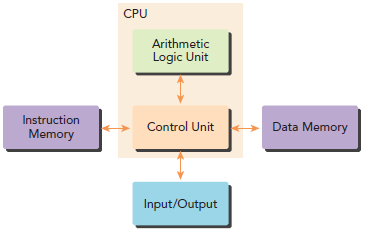
\includegraphics[width=.5\textwidth]{Immagini/CUDA/Harvard_architecture}
	\caption{Architettura Harvard \cite{Cheng:ProfessionalCudaProgramming}}
	\label{fig:Harvard_architecture}
\end{figure}
La componente chiave nell'elaborazione è la CPU, generalmente chiamata core. Al giorno d'oggi, la tendenza nella progettazione dei chip è quella di integrare più core in un singolo processore, generalmente definito multicore, per supportare il parallelismo a livello di architettura. Pertanto, la programmazione può essere vista come il processo di mappatura del calcolo di un problema ai core disponibili in modo tale da ottenere l'esecuzione parallela.

Quando si implementa un algoritmo sequenziale, potrebbe non essere necessario comprendere i dettagli dell'architettura del computer per scrivere un programma corretto. Tuttavia, quando si implementano algoritmi per macchine multicore, è molto più importante che i programmatori siano consapevoli delle caratteristiche dell'architettura del computer sottostante. La scrittura di programmi paralleli sia corretti che efficienti richiede una conoscenza fondamentale delle architetture multicore.
\subsection{Calcolo sequenziale e parallelo}
Quando si scrive un programma, è naturale dividere il problema in una serie discreta di calcoli; ogni calcolo esegue un'attività specifica, come mostrato in Figura~\ref{fig:Execution_order_sequential}. Questo tipo di programma è chiamato \emph{sequenziale}.
\begin{figure}[h!]
	\centering
	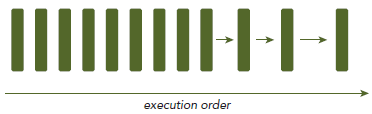
\includegraphics[width=.5\textwidth]{Immagini/CUDA/Execution_order_sequential}
	\caption{Ordine di esecuzione sequenziale \cite{Cheng:ProfessionalCudaProgramming}}
	\label{fig:Execution_order_sequential}
\end{figure}
Esistono due modi per classificare la relazione tra due pezzi di codice: alcuni sono
correlati da un vincolo di precedenza e pertanto devono essere calcolati in sequenza; altri non hanno tali restrizioni e possono essere calcolati contemporaneamente. Qualsiasi programma contenente attività eseguite contemporaneamente è chiamato \emph{parallelo}. Come mostrato in Figura~\ref{fig:Execution_order_parallel}, un programma parallelo può avere alcune parti sequenziali.
\begin{figure}[H]
	\centering
	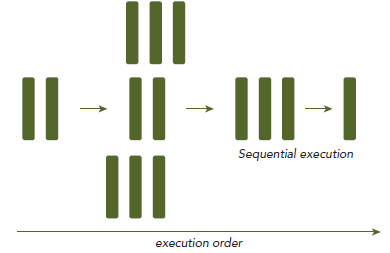
\includegraphics[width=.5\textwidth]{Immagini/CUDA/Execution_order_parallel}
	\caption{Ordine di esecuzione parallelo \cite{Cheng:ProfessionalCudaProgramming}}
	\label{fig:Execution_order_parallel}
\end{figure}
\subsection{Struttura di programmazione CUDA}
Il modello di programmazione CUDA consente di eseguire applicazioni su sistemi di elaborazione eterogenei semplicemente annotando il codice con una piccola serie di estensioni al linguaggio di programmazione C. Un ambiente eterogeneo è costituito da CPU integrate da GPU, ognuna con la propria memoria separata da un bus PCI-Express. Pertanto, è necessario notare la seguente distinzione:
\begin{itemize}
	\item \textbf{Host}: la CPU e la sua memoria (host memory)
	\item \textbf{Device}: la GPU e la sua memoria (device memory)
\end{itemize}
Un componente chiave del modello di programmazione CUDA è il kernel, cioè il codice che viene eseguito sul device GPU. CUDA gestisce i kernel scritti dai programmatori su thread GPU. Dall'host, si definisce il modo in cui l'algoritmo viene mappato sul device in base ai dati dell'applicazione e alla capacità del device GPU. 

L'host può funzionare indipendentemente dal dispositivo per la maggior parte delle operazioni. Quando si chiama un kernel, il controllo viene immediatamente restituito all'host, liberando la CPU per eseguire task aggiuntivi. Un tipico programma CUDA è costituito da un codice seriale integrato da un codice parallelo. Come mostrato in Figura~\ref{fig:Cuda_programming_structure}, il codice seriale (così come quello parallelo) viene eseguito sull'host, mentre il codice parallelo viene eseguito sul device. Il codice del device è scritto usando CUDA C. È possibile inserire tutto il codice in un singolo file sorgente oppure utilizzare più file sorgente per creare l'applicazione o le librerie. Il compilatore NVIDIA C (nvcc) genera il codice eseguibile sia per l'host che per il device.
\begin{figure}[H]
	\centering
	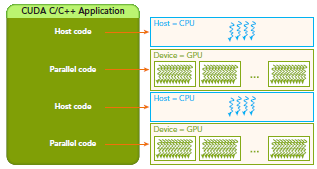
\includegraphics[width=.75\textwidth]{Immagini/CUDA/Cuda_programming_structure}
	\caption{Struttura di programmazione Cuda \cite{Cheng:ProfessionalCudaProgramming}}
	\label{fig:Cuda_programming_structure}
\end{figure}

Un flusso di elaborazione tipico di un programma CUDA segue questo modello:
\begin{enumerate}
	\item Copia i dati dalla memoria della CPU alla memoria della GPU.
	\item Chiama i kernel per operare sui dati memorizzati nella memoria della GPU.
	\item Copia i dati dalla memoria della GPU alla memoria della CPU.
\end{enumerate}
\subsection{Organizzazione della memoria}
\label{sec:managing_memory}
Il modello di programmazione CUDA presuppone un sistema composto da un host e un device, ognuno con una propria memoria separata. I kernel funzionano con la memoria del device. Per consentire il pieno controllo e ottenere le migliori prestazioni, CUDA fornisce funzioni per allocare la memoria del dispositivo, liberare la memoria del dispositivo e trasferire i dati tra la memoria host e quella device. La Tabella~\ref{table:Host and Device Memory Functions} elenca le funzioni C standard e le corrispondenti funzioni CUDA C per le operazioni sulla memoria.
\begin{table}[h!]
	\centering
	\begin{tabular}{c c} 
		\hline
		FUNZIONI C STANDARD & FUNZIONI CUDA C\\
		\hline
		malloc & cudaMalloc\\
		\hline
		memcpy & cudaMemcpy\\
		\hline
		memset & cudaMemset\\
		\hline
		free & cudaFree\\
		\hline
	\end{tabular}
	\caption{Funzioni sulla memoria host e device}
	\label{table:Host and Device Memory Functions}
\end{table}
La funzione utilizzata per eseguire l'allocazione della memoria GPU è cudaMalloc e la sua struttura è:
\begin{lstlisting}[label=code:cudaMalloc_def]
cudaError_t cudaMalloc ( void** devPtr, size_t size )
\end{lstlisting}
Questa funzione alloca un intervallo lineare di memoria del dispositivo con la \emph{size} specificata in byte. La memoria allocata viene restituita tramite \emph{devPtr}. La somiglianza tra cudaMalloc e la libreria runtime standard malloc è intenzionale e ha lo scopo di mantenere l'interfaccia il più vicino possibile alle librerie di runtime C standard.

La funzione utilizzata per trasferire i dati tra l'host e il device è: cudaMemcpy e la sua struttura è:
\begin{lstlisting}[label=code:cudaMemcpy_def]
cudaError_t cudaMemcpy ( void* dst, const void* src, size_t count, cudaMemcpyKind kind )
\end{lstlisting}
Questa funzione copia i byte specificati dall'area di memoria di origine, indicata da \emph{src}, nell'area di memoria di destinazione, indicata da \emph{dst}, con la direzione specificata dal tipo, dove \emph{kind} assume uno dei seguenti tipi:
\begin{itemize}
	\item cudaMemcpyHostToHost
	\item cudaMemcpyHostToDevice
	\item cudaMemcpyDeviceToHost
	\item cudaMemcpyDeviceToDevice
\end{itemize}
Questa funzione mostra un comportamento sincrono perché l'applicazione host si blocca fino a quando cudaMemcpy ritorna e il trasferimento è completo. Ogni chiamata CUDA, ad eccezione del lancio del kernel, restituisce un codice di errore di tipo enumerato cudaError\_t. Ad esempio, se la memoria GPU è allocata correttamente, restituisce:

\textit{cudaSuccess}\\
Altrimenti, ritorna:

\textit{cudaErrorMemoryAllocation}
È possibile convertire un codice di errore in un messaggio di errore human-readable con la seguente funzione di runtime CUDA:
\begin{lstlisting}[label=code:cudaGetErrorString_def]
char* cudaGetErrorString(cudaError_t error)
\end{lstlisting}

La funzione cudaGetErrorString è analoga alla funzione standard C strerror.
Il modello di programmazione CUDA espone un'astrazione della gerarchia di memoria dall'architettura GPU. La Figura~\ref{fig:GPU_Memory_Structure} illustra una struttura di memoria GPU semplificata, contenente due ingredienti principali: global memory e shared memory. Un approfondimento sulla gerarchia di memoria della GPU è presente nel capitolo~\ref{sec:CUDA Memory Model}.
\begin{figure}[h!]
	\centering
	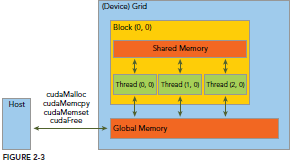
\includegraphics[width=.85\textwidth]{Immagini/CUDA/GPU_Memory_Structure}
	\caption{Struttura della memoria GPU \cite{Cheng:ProfessionalCudaProgramming}}
	\label{fig:GPU_Memory_Structure}
\end{figure}
Una delle caratteristiche più notevoli del modello di programmazione CUDA è la gerarchia di memoria esposta. Ogni dispositivo GPU ha un set di diversi tipi di memoria utilizzati per scopi diversi. Un approfondimento su questa gerarchia è presente nel capitolo~~\ref{sec:CUDA Memory Model}. La global memory è analoga alla memoria di sistema della CPU, mentre la shared memory è simile alla cache della CPU. Tuttavia, la shared memory può essere controllata direttamente da un kernel CUDA C.

\subsection{Organizzazione dei thread}
Quando un kernel viene avviata dal lato host, l'esecuzione viene spostata sul device in cui viene generato un numero elevato di thread e ogni thread esegue le istruzioni specificate dalla funzione kernel. Saper organizzare i thread è una parte fondamentale della programmazione CUDA che espone un'astrazione della gerarchia di thread per consentire di organizzare i thread. Questa è una gerarchia di thread a due livelli composta in blocchi di thread e griglie di blocchi, come mostrato in Figura~\ref{fig:Thread_hierarchy}.
\begin{figure}[h!]
	\centering
	\includegraphics[width=.7\textwidth]{Immagini/CUDA/Thread_hierarchy}
	\caption{Thread hierarchy \cite{Cheng:ProfessionalCudaProgramming}}
	\label{fig:Thread_hierarchy}
\end{figure}
Tutti i thread generati da un singolo lancio del kernel sono collettivamente chiamati griglia. Tutti i thread in una griglia condividono lo stesso spazio di global memory. Una griglia è composta da molti blocchi di thread. Un blocco thread è un gruppo di thread che possono cooperare tra loro usando:
\begin{itemize}
	\item sincronizzazione dei blocchi locali
	\item shared memory dei blocchi locali
\end{itemize}
Threads da blocchi diversi non possono cooperare. I threads si basano sulle seguenti due coordinate univoche per distinguersi l'una dall'altra:
\begin{itemize}
	\item blockIdx (indice del blocco all'interno di una griglia)
	\item threadIdx (indice del thread all'interno di un blocco)
\end{itemize}
Queste variabili appaiono come variabili predefinite pre-inizializzate a cui è possibile accedere nei kernel. Quando viene eseguita un kernel, le variabili di coordinate blockIdx e threadIdx vengono assegnate a ciascun thread dal CUDA runtime. Sulla base delle coordinate, è possibile assegnare porzioni di dati a thread diversi.

La variabile di coordinate è di tipo uint3. È una struttura contenente tre numeri interi senza segno e la prima, seconda e terza componente è accessibile attraverso i campi x, y e z.

blockIdx.x

blockIdx.y

blockIdx.z

threadIdx.x

threadIdx.y

threadIdx.z

CUDA organizza griglie e blocchi in tre dimensioni. La Figura~\ref{fig:Thread_hierarchy} mostra un esempio di una struttura gerarchica di thread con una griglia 2D contenente blocchi 2D. Le dimensioni di una griglia e di un blocco sono specificate dalle seguenti due variabili integrate:
\begin{itemize}
	\item blockDim (dimensione del blocco, misurata in threads)
	\item gridDim (dimensione della griglia, misurata in blocchi)
\end{itemize}
Queste variabili sono di tipo dim3, un tipo di vettore intero basato su uint3 utilizzato per specificare le dimensioni. Quando si definisce una variabile di tipo dim3, qualsiasi componente lasciato non specificato viene inizializzato su 1. Ogni componente in una variabile di tipo dim3 è accessibile attraverso i suoi campi x, y e z, rispettivamente, come mostrato dai campi mostrati di seguito:

blockDim.x

blockDim.y

blockDim.z
\subsection{Modello della memoria CUDA}
\label{sec:CUDA Memory Model}
Per i programmatori, ci sono generalmente due classificazioni di memoria:
\begin{itemize}
	\item Programmabile: si controlla esplicitamente quali dati vengono inseriti nella memoria programmabile.
	\item Non programmabile: non si ha alcun controllo sul posizionamento dei dati e si fa affidamento su tecniche automatiche per ottenere buone prestazioni.
\end{itemize}
Nella gerarchia di memoria della CPU, la cache L1 e la cache L2 sono esempi di memoria non programmabile. CUDA espone molti tipi di memoria programmabile:
\begin{itemize}
	\item Registers
	\item Shared memory
	\item Local memory
	\item Constant memory
	\item Texture memory
	\item Global memory
\end{itemize}
La Figura~\ref{fig:GPU_Memory_Hierarchy} illustra la gerarchia di questi spazi di memoria. Ognuno ha un diverso ambito, durata e comportamento di memorizzazione nella cache.
\begin{figure}[h!]
	\centering
	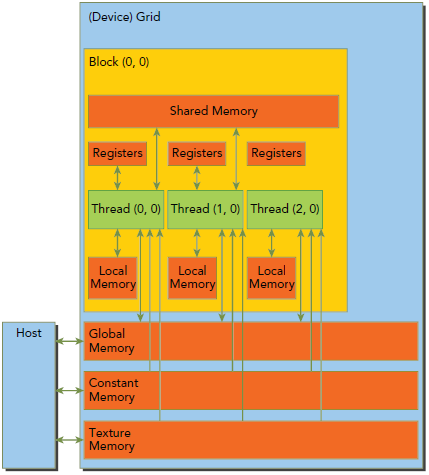
\includegraphics[width=.7\textwidth]{Immagini/CUDA/GPU_Memory_Hierarchy}
	\caption{Gerarchia della memoria della GPU \cite{Cheng:ProfessionalCudaProgramming}}
	\label{fig:GPU_Memory_Hierarchy}
\end{figure}
Un thread in un kernel ha la sua local memory privata. Un blocco di thread ha una propria memoria shared, visibile a tutti i thread nello stesso blocco thread e il cui contenuto persiste per la durata del blocco thread. Tutti i thread possono accedere alla memoria globale. Esistono anche due spazi di memoria di sola lettura accessibili da tutti i thread: la memoria costante e texture. Gli spazi di memoria globale, costante e texture sono ottimizzati per usi diversi. La Texture memory offre diverse modalità di indirizzo. I contenuti della memoria globale, costante e texture hanno la stessa durata di un'applicazione.
\subsubsection{Registri}
I registri sono lo spazio di memoria più veloce su una GPU. Una variabile dichiarata in un kernel senza altri qualificatori di tipo viene generalmente memorizzata in un registro. Le matrici dichiarate in un kernel possono anche essere memorizzate in registri, ma solo se gli indici utilizzati per fare riferimento alla matrice sono costanti e possono essere determinati al momento della compilazione.

Le variabili nei registri sono private per ogni thread. Un kernel in genere usa i registri per contenere variabili thread private a cui si accede frequentemente. Le variabili nei registri condividono la loro durata con il kernel. Una volta che un kernel ha completato l'esecuzione, non è possibile accedere nuovamente a una variabile nel registro.

I registri sono risorse scarse che vengono suddivise tra gli warp attivi nella Shared Memory (SM).

\subsubsection{Local Memory}
Le variabili in un kernel idonee per i registri ma che non possono rientrare nello spazio di registro allocato per quel kernel si riverseranno nella memoria locale. Le variabili che è probabile che il compilatore inserisca nella memoria locale sono:
\begin{itemize}
	\item Array locali referenziate con indici i cui valori non possono essere determinati in fase di compilazione.
	\item Grandi strutture locali o array che consumerebbero troppo spazio sui registri.
	\item Qualsiasi variabile che non rientra nel limite del registro del kernel.
\end{itemize}
Il nome "memoria locale" è fuorviante: i valori riversati nella memoria locale risiedono nella stessa posizione fisica della memoria globale, quindi gli accessi alla memoria locale sono caratterizzati da elevata latenza e bassa larghezza di banda e sono soggetti ai requisiti per un accesso efficiente alla memoria.

\subsubsection{Shared Memory}
Le variabili con il seguente attributo in un kernel sono immagazzinate nella memoria condivisa:

\_\_shared\_\_ \\

Poiché la shared memory è su chip, ha una larghezza di banda molto più elevata e una latenza molto inferiore rispetto alla memoria locale o globale. È usato in modo simile alla cache L1 della CPU, ma è anche programmabile.

Ogni SM ha una quantità limitata di memoria condivisa che è partizionata tra i blocchi di thread. Pertanto, è necessario fare attenzione a non utilizzare eccessivamente la memoria condivisa o si limiterà inavvertitamente il numero di orditi attivi.

La memoria condivisa è dichiarata nell'ambito di una funzione del kernel ma condivide la sua durata con un blocco di thread. Quando viene eseguito il blocco, la sua allocazione di memoria condivisa verrà rilasciata e assegnata ad altri blocchi thread.

La shared memory serve come mezzo di base per la comunicazione tra thread. I thread all'interno di un blocco possono cooperare condividendo i dati memorizzati nella memoria condivisa. L'accesso alla shared memory deve essere sincronizzato utilizzando la seguente chiamata:
\begin{lstlisting}[label=code:syncthreads_def]
void __syncthreads();
\end{lstlisting}
Questa funzione crea una barriera che tutti i thread nello stesso blocco di thread devono raggiungere prima di poter procedere con qualsiasi altro thread. Creando una barriera per tutti i thread all'interno di un blocco, è possibile prevenire un potenziale rischio di dati. Si verificano quando esiste un ordinamento indefinito di accessi multipli nella stessa posizione di memoria da thread diversi, in cui almeno uno di questi accessi è una scrittura. \_syncthreads può anche influire sulle prestazioni costringendo la SM a rimanere inattiva frequentemente.

\subsubsection{Constant Memory}
La memoria costante risiede nella memoria del device ed è memorizzata nella cache costante dedicata per la SM. Una variabile costante ha il seguente attributo:

\_\_constant\_\_ \\

Le variabili costanti devono essere dichiarate globalmente, al di fuori di qualsiasi kernel. È possibile dichiarare una quantità limitata di memoria costante: 64 KB. La memoria costante viene dichiarata staticamente ed è visibile a tutti i kernel.

I kernel possono sololeggere  dalla memoria costante che deve quindi essere inizializzata dall'host utilizzando:
\begin{lstlisting}[label=code:cudaMemcpyToSymbol_def]
cudaError_t cudaMemcpyToSymbol(const void* symbol, const void* src, size_t count);
\end{lstlisting}
Questa funzione copia i byte di conteggio dalla memoria a cui punta \emph{src} alla memoria a cui punta il simbolo, che è una variabile che risiede sul dispositivo nella memoria globale o costante. Questa funzione è sincrona nella maggior parte dei casi.

La memoria costante funziona meglio quando tutti i thread in un warp leggono dallo stesso indirizzo di memoria. Ad esempio, è opportuno scrivere un coefficiente per una formula matematica nella memoria costante perché tutti i thread useranno lo stesso numero per condurre lo stesso calcolo su dati diversi. Se ogni thread in un warp legge da un indirizzo diverso e legge solo una volta, la memoria costante non è la scelta migliore perché una sola lettura dalla memoria costante si trasmette a tutti i thread in un warp.

\subsubsection{Texture Memory}
La memoria texture si trova nella memoria del device ed è memorizzata in una cache di sola lettura per SM. È un tipo di memoria globale a cui si accede tramite una cache di sola lettura dedicata che include il supporto per il filtro hardware, che può eseguire l'interpolazione in virgola mobile. La memoria texture è ottimizzata per spazi 2D, quindi i thread in un warp che la utilizzano per accedere ai dati 2D otterranno le migliori prestazioni. Per alcune applicazioni, questo è l'ideale e offre un vantaggio in termini di prestazioni grazie alla cache e all'hardware di filtro. Tuttavia, per altre applicazioni l'utilizzo della memoria texture può essere più lento della memoria globale.

\subsubsection{Global Memory}
La memoria globale è la memoria più grande, a più alta latenza e più comunemente usata su una GPU. Il nome \emph{global} si riferisce alla sua portata e durata. È possibile accedere al suo stato sul device per tutta la durata dell'applicazione.

Una variabile nella memoria globale può essere dichiarata staticamente o dinamicamente. Si può dichiarare staticamente una variabile globale nel codice del dispositivo usando il seguente qualificatore:
\_\_device\_\_\\

Nel Capitolo~\ref{sec:managing_memory}, si è definito come allocare dinamicamente la memoria globale dall'host utilizzando cudaMalloc e liberata utilizzando cudaFree. I puntatori alla memoria globale vengono quindi passati alle funzioni del kernel come parametri. Le allocazioni di memoria globale esistono per la durata di un'applicazione e sono accessibili a tutti i thread di tutti i kernel. È necessario prestare attenzione quando si accede alla memoria globale da più thread. Poiché non è possibile sincronizzare l'esecuzione di thread tra blocchi di thread, esiste il potenziale rischio che più thread in blocchi diversi modifichino contemporaneamente la stessa posizione nella memoria globale, il che porterà a un comportamento del programma indefinito.

La memoria globale risiede nella memoria del dispositivo ed è accessibile tramite transazioni di memoria a 32, 64 o 128 byte. Queste transazioni devono essere allineate, cioè il primo indirizzo deve essere un multiplo di 32 byte, 64 byte o 128 byte. L'ottimizzazione delle transazioni di memoria è fondamentale per ottenere prestazioni ottimali. Quando un warp esegue una operazione load/store, il numero di transazioni richieste per soddisfare quella richiesta dipende in genere dai seguenti due fattori:
\begin{itemize}
	\item Distribuzione degli indirizzi di memoria tra i thread del warp.
	\item Allineamento degli indirizzi di memoria per transazione.
\end{itemize}
In generale, maggiore è il numero di transazioni necessarie per soddisfare una richiesta di memoria, maggiore è il potenziale di trasferimento di byte non utilizzati, con conseguente riduzione dell'efficienza del throughput.